\section{Clustering of Influenza} \label{sec:Clustering}

From each of the four different pipelines the execution results in a CSV file containing the used values settings and a summary of the clustering. Every segment of \gls{IAV} was clustered by each method, resulting in the tables having 8 rows representing the segments. By comparing the tabls of \gls{PCA} and \gls{UMAP} with the same $\varepsilon$ exploration by the Kneedle Algorithm (\autoref{tab:PCA_Cluster_Knee} and \autoref{tab:UMAP_Cluster_Knee}) a major difference in the number of raw and final cluster stand out. The number of clusters found by hybrid \gls{HDBSCAN} with only \gls{PCA} reduced k-mer vectors is around 60 to 70 in the raw clustering with the $\varepsilon$ treshhold defined by the Kneedle Algorithm. By \glspl{HDBSCAN} adjustment for points not affected by the threshold $\varepsilon$ the number is decreased to around 40 to 50 cluster per segment. The final amount of clusters per segment is a number hoped for from the beginning, since investigation is feasible in an appropriate amount of time and also relativ close to the state of the art subtype classification with 18 \gls{HA} and 11 \gls{NA} antibody subtypes \autocite{noauthor_revision_1980}. The \gls{UMAP} method with the Kneedle Algorithm offers a way higher number of clusters with no difference of raw and final cluster number. This can be explained by the overall higher $\varepsilon$ threshold compared to the \gls{PCA} version. By a higher $\varepsilon$ more points are affected by this threshold and therefore the chance that all points are included by the \gls{DBSCAN} part of the hybrid \gls{HDBSCAN} increases. When all points are affected by the $\varepsilon$ \gls{DBSCAN} threshold no final adjustment with \gls{HDBSCAN} is performed. Still the number of clusters is way higher than with \gls{PCA} only and a accurate investigation is much more time-consuming, furthermore around 250 clusters are difficult to use for a possible new classification. In addition to that it is necessary to point out the lower number of unclustered sequences with \gls{UMAP}, which is in fact zero with every segment. The approach using \gls{PCA} alone is unable to cluster around 10 to 30 sequences per segment. However the number of unclustered for e.~ g.~ segment 4 is 6 of 56617 used sequences and therefore $\approx$ 0.01\%. As a comparison 1191 sequences segment 4 are declared unclassified by the subtype convention making $\approx$ 2\%. 

\begin{table}[!hbt]
    \centering
    \caption[Knee based Clustering (\Acrshort{PCA})]{\textbf{Knee based Clustering (\Acrshort{PCA}).}.}
    \label{tab:PCA_Cluster_Knee}
    \pgfplotstabletypeset[
        every head row/.style={
            before row={
                \toprule
                & \multicolumn{3}{l}{\textbf{Cluster}} &  & \multicolumn{2}{l}{\textbf{mixed}} &\\
                \cmidrule(lr){2-4}\cmidrule(lr){6-7}
            },
            after row={
                \midrule
            },
        },
        every last row/.style={
            after row={
                %... & ... & ... & ... & ... & ... & ... & ...\\
                \bottomrule
            },
        },
        begin table=\begin{tabular*}{\textwidth},
        end table=\end{tabular*},
        columns={0,1,2,3,4,5,6,7,8},
        columns/0/.style={int detect, multicolumn names=l,column name=\textbf{Segment}, column type=@{\extracolsep{\fill}\hspace{6pt}}r},
        columns/1/.style={int detect, multicolumn names=l,column name=\textbf{\#Final}, column type=r},
        columns/2/.style={int detect, multicolumn names=l,column name=\textbf{\#Raw}, column type=r},
        columns/3/.style={multicolumn names=l,column name=\textbf{Normalized}, column type=r},
        columns/4/.style={int detect, multicolumn names=l,column name=\textbf{\#Unclustered}, column type=r},
        columns/5/.style={int detect, multicolumn names=l,column name=\textbf{H}, column type=r},
        columns/6/.style={int detect, multicolumn names=l,column name=\textbf{N}, column type=r},
        columns/7/.style={multicolumn names=l,column name=\textbf{$\varepsilon$}, column type=r},
        columns/8/.style={multicolumn names=l,column name=\textbf{Variance}, column type=r},
    ]
    {PCA/information.csv}
\end{table}

\begin{table}[!hbt]
    \centering
    \caption[Knee based Clustering (\Acrshort{UMAP})]{\textbf{Knee based Clustering (\Acrshort{UMAP}).}.}
    \label{tab:UMAP_Cluster_Knee}
    \pgfplotstabletypeset[
        every head row/.style={
            before row={
                \toprule
                & \multicolumn{3}{l}{\textbf{Cluster}} &  & \multicolumn{2}{l}{\textbf{mixed}} &\\
                \cmidrule(lr){2-4}\cmidrule(lr){6-7}
            },
            after row={
                \midrule
            },
        },
        every last row/.style={
            after row={
                %... & ... & ... & ... & ... & ... & ... & ...\\
                \bottomrule
            },
        },
        begin table=\begin{tabular*}{\textwidth},
        end table=\end{tabular*},
        columns={0,1,2,3,4,5,6,7,8},
        columns/0/.style={int detect, multicolumn names=l,column name=\textbf{Segment}, column type=@{\extracolsep{\fill}\hspace{6pt}}r},
        columns/1/.style={int detect, multicolumn names=l,column name=\textbf{\#Final}, column type=r},
        columns/2/.style={int detect, multicolumn names=l,column name=\textbf{\#Raw}, column type=r},
        columns/3/.style={multicolumn names=l,column name=\textbf{Normalized}, column type=r},
        columns/4/.style={int detect, multicolumn names=l,column name=\textbf{\#Unclustered}, column type=r},
        columns/5/.style={int detect, multicolumn names=l,column name=\textbf{H}, column type=r},
        columns/6/.style={int detect, multicolumn names=l,column name=\textbf{N}, column type=r},
        columns/7/.style={multicolumn names=l,column name=\textbf{$\varepsilon$}, column type=r},
        columns/8/.style={multicolumn names=l,column name=\textbf{Variance}, column type=r},
    ]
    {UMAP/information.csv}
\end{table}

Comparing the methods to the ones using the \gls{DBCV} for $\varepsilon$ exploration instead of the Kneedle Algorithm (\autoref{tab:PCA_Cluster_DBCV} and \autoref{tab:UMAP_Cluster_DBCV}) there doesn't seem to be much difference for \gls{UMAP} with \gls{DBCV} method. The overall $\varepsilon$ threshold found by the \gls{DBCV} is a little smaller and therefore the number of clusters a little higher compared to the results found with $\varepsilon$ by the Kneedle Algorithm. Using \gls{DBCV} to find the optimal $\varepsilon$ with the \gls{PCA} pipeline on the other hand changes the results drastically. The number of final clusters is between 9000 and 12000 depending on the segment, with the exception of segment 4. The raw cluster number is equivalent to the total number of sequences for the given segment. Also the number of unclustered sequences is increased by a major amount to around 20\% for some segments. Only the clustering of segment 4 with \gls{DBCV} $\varepsilon$ exploration seems to be as stable as with the Kneedle Algorithm. The number of clusters for the other segments is higher, because the \gls{DBCV} method is searching for the $\varepsilon$ value setting that results in the best \gls{DBCV}, which is for most segments a setting of zero. Hybrid clustering with a $\varepsilon$ value of zero is standard \gls{HDBSCAN} and as mentioned in \autoref{sec:HDBSCAN} not suited for \gls{IAV} clustering without the hybrid \gls{DBSCAN} component. Based on the tables \autoref{tab:PCA_Cluster_Knee}, \autoref{tab:UMAP_Cluster_Knee}, \autoref{tab:PCA_Cluster_DBCV} and \autoref{tab:UMAP_Cluster_DBCV} it appears that the only the combination of \gls{PCA} and the Kneedle Algorithm results in an appropriate number of clusters for every segment. Further investigation on the details of the parameters is done in the following.

\begin{table}[!hbt]
    \centering
    \caption[\Acrshort{DBCV} based Clustering (\Acrshort{PCA})]{\textbf{\Acrshort{DBCV} based Clustering (\Acrshort{PCA}).}.}
    \label{tab:PCA_Cluster_DBCV}
    \pgfplotstabletypeset[
        every head row/.style={
            before row={
                \toprule
                & \multicolumn{2}{l}{\textbf{Cluster}} &  & \multicolumn{2}{l}{\textbf{mixed}} & &\\
                \cmidrule(lr){2-3}\cmidrule(lr){5-6}
            },
            after row={
                \midrule
            },
        },
        every last row/.style={
            after row={
                %... & ... & ... & ... & ... & ... & ... & ...\\
                \bottomrule
            },
        },
        begin table=\begin{tabular*}{\textwidth},
        end table=\end{tabular*},
        columns={0,1,2,3,4,5,6,7,8},
        columns/0/.style={int detect, multicolumn names=l,column name=\textbf{Segment}, column type=@{\extracolsep{\fill}\hspace{6pt}}r},
        columns/1/.style={int detect, multicolumn names=l,column name=\textbf{\#Final}, column type=r},
        columns/2/.style={int detect, multicolumn names=l,column name=\textbf{\#Raw}, column type=r},
        columns/3/.style={int detect, multicolumn names=l,column name=\textbf{\#Unclustered}, column type=r},
        columns/4/.style={int detect, multicolumn names=l,column name=\textbf{H}, column type=r},
        columns/5/.style={int detect, multicolumn names=l,column name=\textbf{N}, column type=r},
        columns/6/.style={multicolumn names=l,column name=\textbf{$\varepsilon$}, column type=r},
        columns/7/.style={multicolumn names=l,column name=\textbf{DBCV}, column type=r},
        columns/8/.style={multicolumn names=l,column name=\textbf{Variance}, column type=r},
    ]
    {PCA/information_alt.csv}
\end{table}

\begin{table}[!hbt]
    \centering
    \caption[\Acrshort{DBCV} based Clustering (\Acrshort{UMAP})]{\textbf{\Acrshort{DBCV} based Clustering (\Acrshort{UMAP}).}.}
    \label{tab:UMAP_Cluster_DBCV}
    \pgfplotstabletypeset[
        every head row/.style={
            before row={
                \toprule
                & \multicolumn{2}{l}{\textbf{Cluster}} &  & \multicolumn{2}{l}{\textbf{mixed}} & &\\
                \cmidrule(lr){2-3}\cmidrule(lr){5-6}
            },
            after row={
                \midrule
            },
        },
        every last row/.style={
            after row={
                %... & ... & ... & ... & ... & ... & ... & ...\\
                \bottomrule
            },
        },
        begin table=\begin{tabular*}{\textwidth},
        end table=\end{tabular*},
        columns={0,1,2,3,4,5,6,7,8},
        columns/0/.style={int detect, multicolumn names=l,column name=\textbf{Segment}, column type=@{\extracolsep{\fill}\hspace{6pt}}r},
        columns/1/.style={int detect, multicolumn names=l,column name=\textbf{\#Final}, column type=r},
        columns/2/.style={int detect, multicolumn names=l,column name=\textbf{\#Raw}, column type=r},
        columns/3/.style={int detect, multicolumn names=l,column name=\textbf{\#Unclustered}, column type=r},
        columns/4/.style={int detect, multicolumn names=l,column name=\textbf{H}, column type=r},
        columns/5/.style={int detect, multicolumn names=l,column name=\textbf{N}, column type=r},
        columns/6/.style={multicolumn names=l,column name=\textbf{$\varepsilon$}, column type=r},
        columns/7/.style={multicolumn names=l,column name=\textbf{DBCV}, column type=r},
        columns/8/.style={multicolumn names=l,column name=\textbf{Variance}, column type=r},
        %row predicate/.code={%
        %    \ifnum#1>0\relax
        %        \ifnum#1<2\relax
        %            \pgfplotstableuserowfalse
        %        \fi
        %    \fi
        %}
    ]
    {UMAP/information_alt.csv}
\end{table}

To finally determine the best combination of methods for clustering \gls{IAV}, the used parameters were visualized for better understanding and analysis. Since investigation of all segments would overfill this section, only the four methods parameters for segment 4 were discussed in detail. Nevertheless all graphics for the other segments with every used method can be found in the \autoref{chap:Appendix}. A big difference in the cluster size distribution stand out, when comparing the methods with \gls{PCA} to the ones with \gls{UMAP}. The sizes of \gls{PCA} clustering consist mostly of very small ones and one or two very big ones with more than 10000 sequences (\autoref{subfig:PCA_Cluster_DBCV_Distribution_4} and \autoref{subfig:PCA_Cluster_Knee_Distributione_4}). 

\begin{figure}[!hbt]
    \centering
    %\begin{adjustbox}{minipage=\dimexpr\textwidth-2\fboxsep-2\fboxrule,fbox}
    \begin{subfigure}[b]{0.475\textwidth}
        \caption[Kneedle Algorithm]{\textbf{Kneedle Algorithm}}
        \label{subfig:UMAP_Cluster_Knee_Kneedle_4}            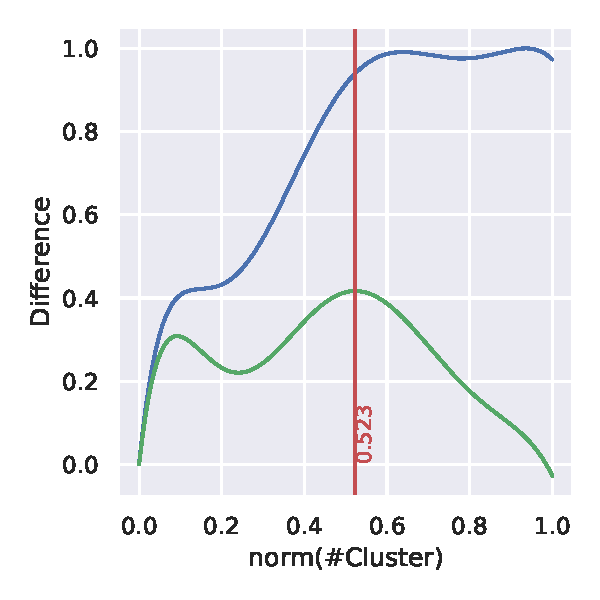
\includegraphics[width=\textwidth]{UMAP/Cluster_Knee_Segment_4.pdf}
    \end{subfigure}
    \hfill
    \begin{subfigure}[b]{0.475\textwidth}
        \caption[Kneedle Knee]{\textbf{Kneedle Knee}}
        \label{subfig:UMAP_Cluster_Knee_Elbow_4}            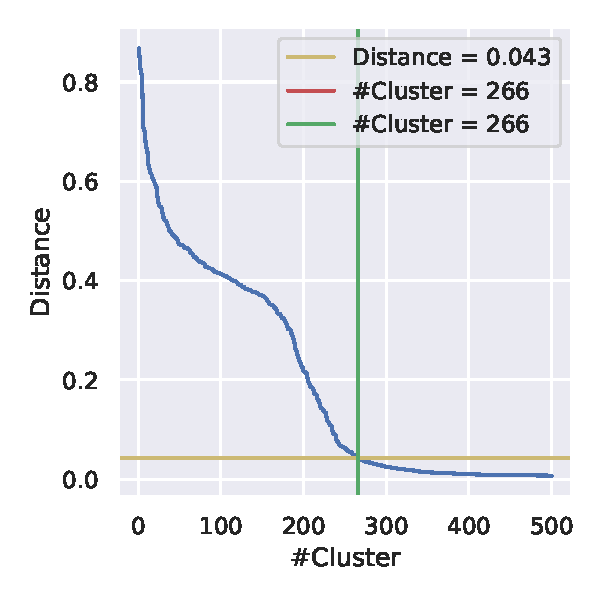
\includegraphics[width=\textwidth]{UMAP/Cluster_Elbow_Knee_Segment_4.pdf}
    \end{subfigure}
    \vskip\baselineskip
    \begin{subfigure}[b]{0.475\textwidth}
        \caption[Cluster Distribution]{\textbf{Cluster Distribution}}
        \label{subfig:UMAP_Cluster_Knee_Distributione_4}            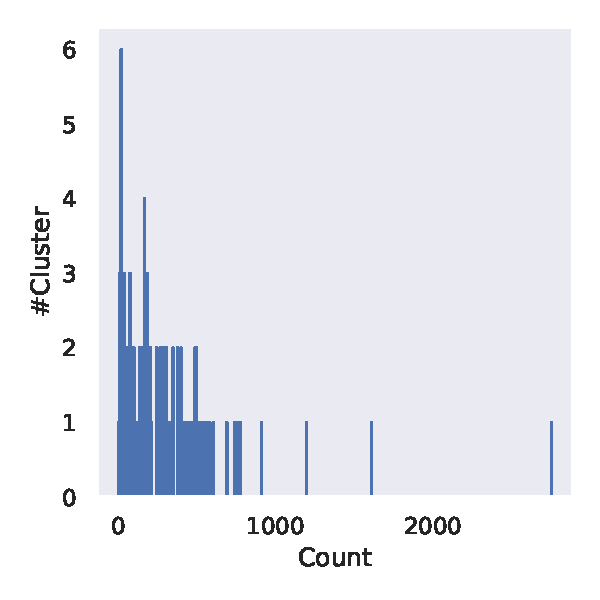
\includegraphics[width=\textwidth]{UMAP/Cluster_Distribution_Segment_4.pdf}
    \end{subfigure}
    \hfill
    \begin{subfigure}[b]{0.475\textwidth}
        \caption[Logarithmic Distribution]{\textbf{Logarithmic Distribution}}
        \label{subfig:UMAP_Cluster_Knee_Distribution_log_4}            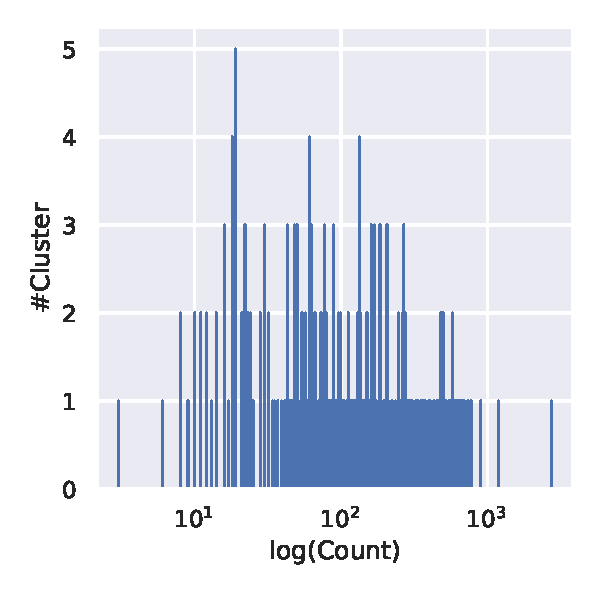
\includegraphics[width=\textwidth]{UMAP/Cluster_Distribution_Log_Segment_4.pdf}
    \end{subfigure}
    %\end{adjustbox}
    \caption[Knee based Segment 4 Clustering (\Acrshort{UMAP})]{\textbf{Knee based Segment 4 Clustering (\Acrshort{UMAP}).}.}
    \label{fig:UMAP_Cluster_Knee_4}
\end{figure}

\begin{figure}[!hbt]
    \centering
    %\begin{adjustbox}{minipage=\dimexpr\textwidth-2\fboxsep-2\fboxrule,fbox}
    \begin{subfigure}[b]{0.475\textwidth}
        \caption[Kneedle Algorithm]{\textbf{Kneedle Algorithm}}
        \label{subfig:PCA_Cluster_Knee_Kneedle_4}            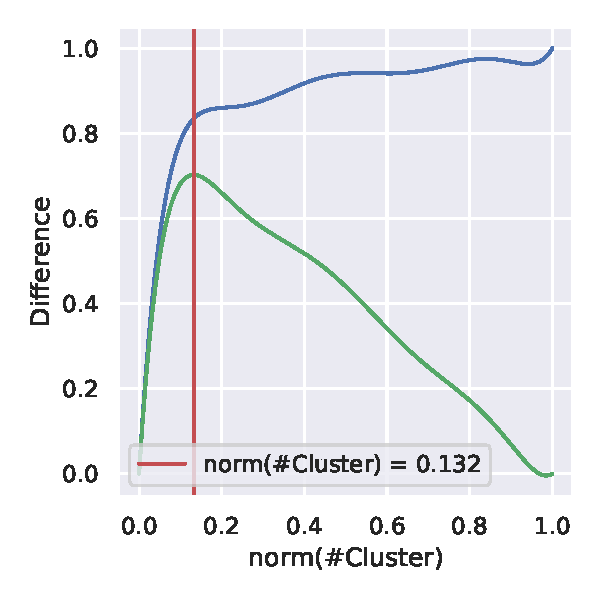
\includegraphics[width=\textwidth]{PCA/Cluster_Knee_Segment_4.pdf}
    \end{subfigure}
    \hfill
    \begin{subfigure}[b]{0.475\textwidth}
        \caption[Kneedle Knee]{\textbf{Kneedle Knee}}
        \label{subfig:PCA_Cluster_Knee_Elbow_4}            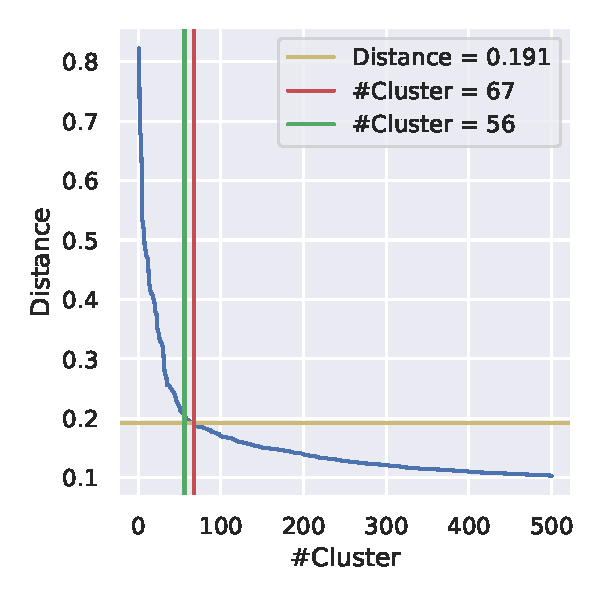
\includegraphics[width=\textwidth]{PCA/Cluster_Elbow_Knee_Segment_4.pdf}
    \end{subfigure}
    \vskip\baselineskip
    \begin{subfigure}[b]{0.475\textwidth}
        \caption[Cluster Distribution]{\textbf{Cluster Distribution}}
        \label{subfig:PCA_Cluster_Knee_Distributione_4}            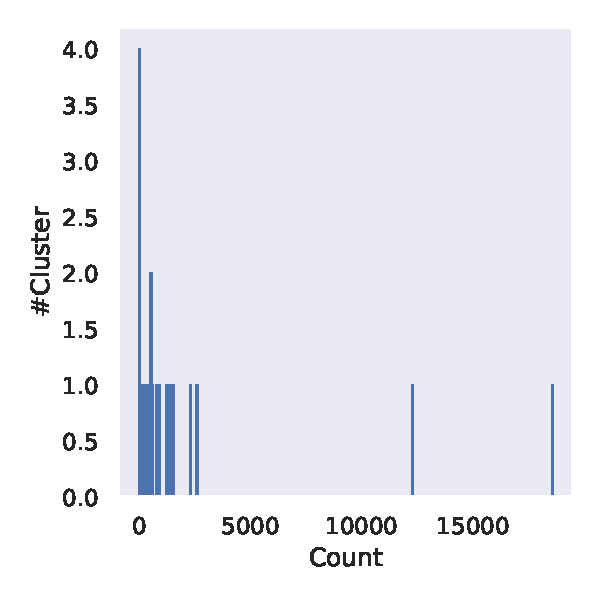
\includegraphics[width=\textwidth]{PCA/Cluster_Distribution_Segment_4.pdf}
    \end{subfigure}
    \hfill
    \begin{subfigure}[b]{0.475\textwidth}
        \caption[Logarithmic Distribution]{\textbf{Logarithmic Distribution}}
        \label{subfig:PCA_Cluster_Knee_Distribution_log_4}            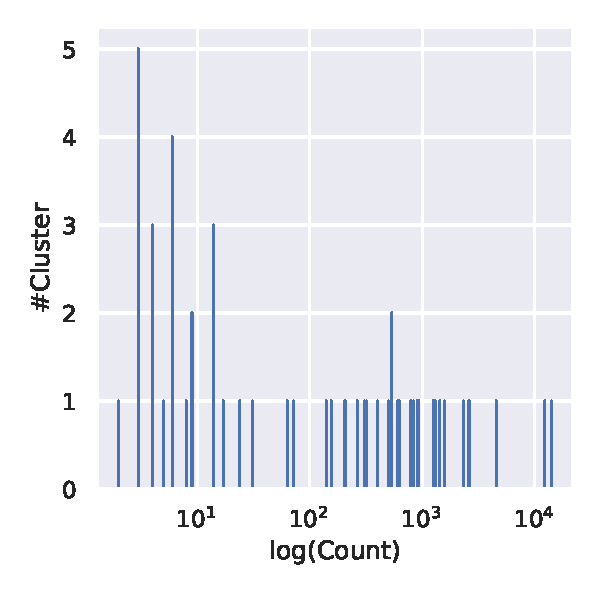
\includegraphics[width=\textwidth]{PCA/Cluster_Distribution_Log_Segment_4.pdf}
    \end{subfigure}
    %\end{adjustbox}
    \caption[Knee based Segment 4 Clustering (\Acrshort{PCA})]{\textbf{Knee based Segment 4 Clustering (\Acrshort{PCA}).}.}
    \label{fig:PCA_Cluster_Knee_4}
\end{figure}

\begin{figure}[!hbt]
    \centering
    %\begin{adjustbox}{minipage=\dimexpr\textwidth-2\fboxsep-2\fboxrule,fbox}
    \begin{subfigure}[b]{0.475\textwidth}
        \caption[\Acrshort{DBCV} Exploration]{\textbf{\Acrshort{DBCV} Exploration}}
        \label{subfig:PCA_Cluster_DBCV_Explo_4}            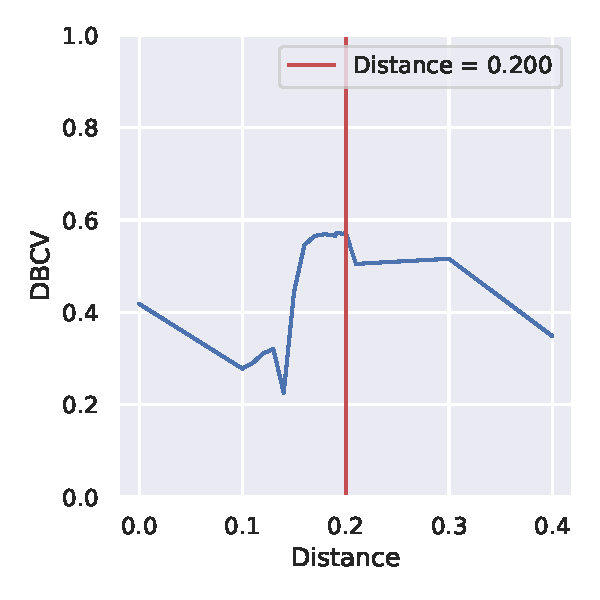
\includegraphics[width=\textwidth]{PCA/Cluster_DBCV_Segment_4.pdf}
    \end{subfigure}
    \hfill
    \begin{subfigure}[b]{0.475\textwidth}
        \caption[\Acrshort{DBCV} Knee]{\textbf{\Acrshort{DBCV} Knee}}
        \label{subfig:PCA_Cluster_DBCV_Elbow_4}            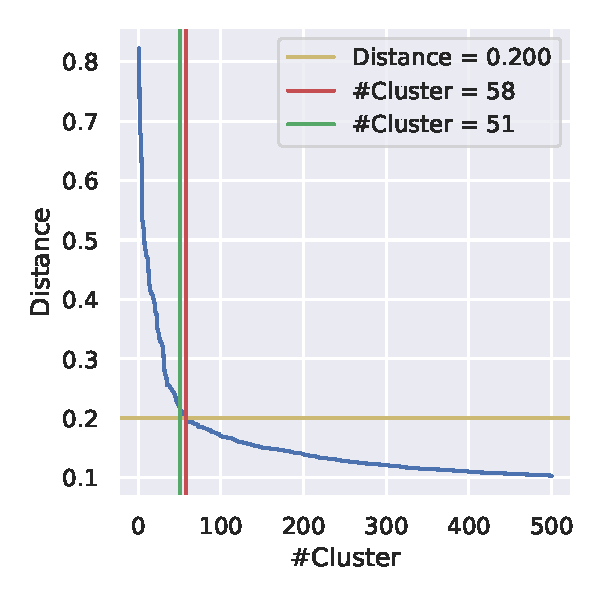
\includegraphics[width=\textwidth]{PCA/Cluster_Elbow_DBCV_Segment_4.pdf}
    \end{subfigure}
    \vskip\baselineskip
    \begin{subfigure}[b]{0.475\textwidth}
        \caption[Cluster Distribution]{\textbf{Cluster Distribution}}
        \label{subfig:PCA_Cluster_DBCV_Distribution_4}            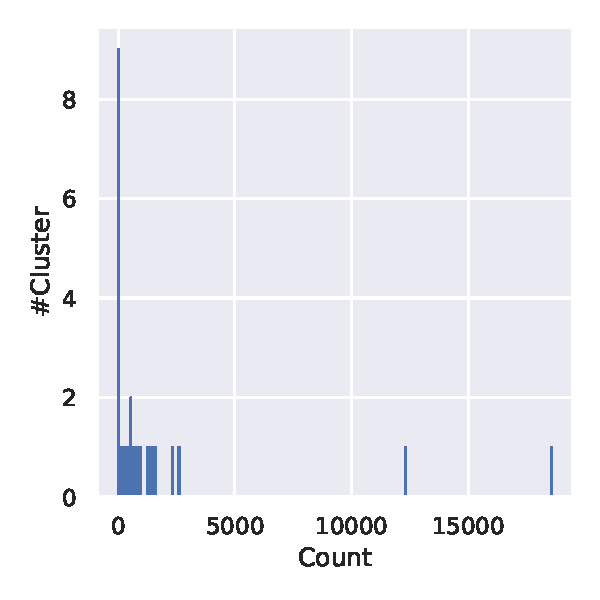
\includegraphics[width=\textwidth]{PCA/Cluster_Distribution_Segment_4_alternative.pdf}
    \end{subfigure}
    \hfill
    \begin{subfigure}[b]{0.475\textwidth}
        \caption[Logarithmic Distribution]{\textbf{Logarithmic Distribution}}
        \label{subfig:PCA_Cluster_DBCV_Distribution_log_4}            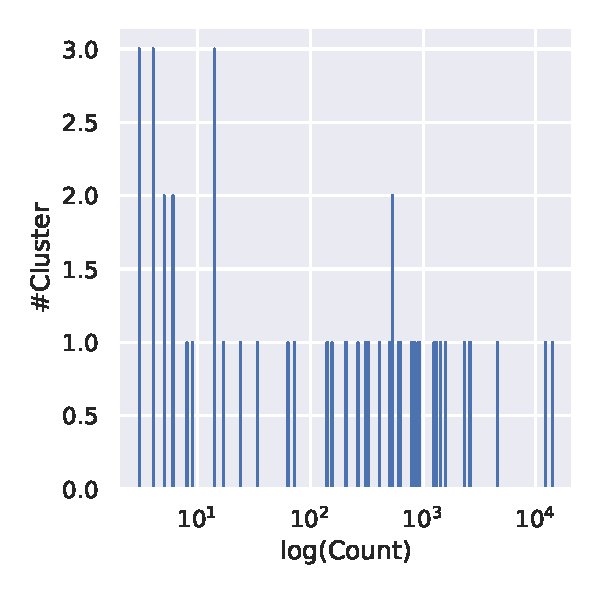
\includegraphics[width=\textwidth]{PCA/Cluster_Distribution_Log_Segment_4_alternative.pdf}
    \end{subfigure}
    %\end{adjustbox}
    \caption[\Acrshort{DBCV} based Segment 4 Clustering (\Acrshort{PCA})]{\textbf{\Acrshort{DBCV} based Segment 4 Clustering (\Acrshort{PCA}).}.}
    \label{fig:PCA_Cluster_DBCV_4}
\end{figure}

\begin{figure}[!hbt]
    \centering
    %\begin{adjustbox}{minipage=\dimexpr\textwidth-2\fboxsep-2\fboxrule,fbox}
    \begin{subfigure}[b]{0.475\textwidth}
        \caption[\Acrshort{DBCV} Exploration]{\textbf{\Acrshort{DBCV} Exploration}}
        \label{subfig:UMAP_Cluster_DBCV_Explo_4}            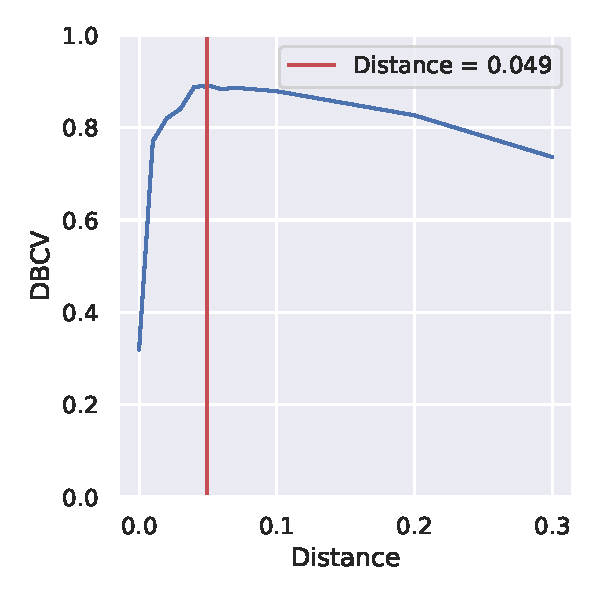
\includegraphics[width=\textwidth]{UMAP/Cluster_DBCV_Segment_4.pdf}
    \end{subfigure}
    \hfill
    \begin{subfigure}[b]{0.475\textwidth}
        \caption[\Acrshort{DBCV} Knee]{\textbf{\Acrshort{DBCV} Knee}}
        \label{subfig:UMAP_Cluster_DBCV_Elbow_4}            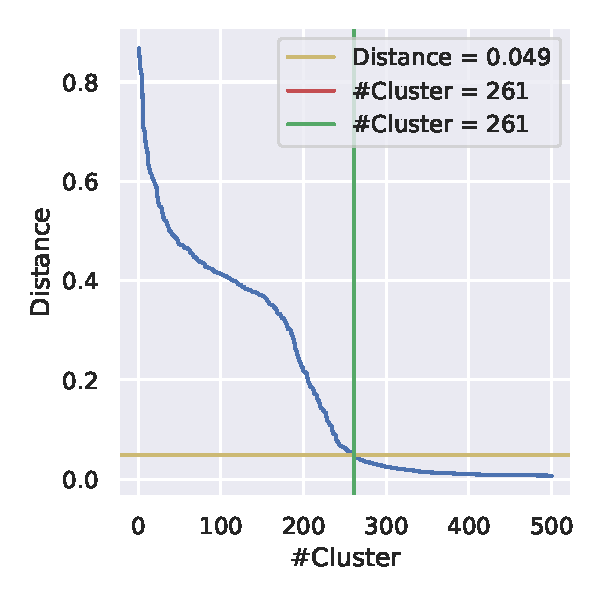
\includegraphics[width=\textwidth]{UMAP/Cluster_Elbow_DBCV_Segment_4.pdf}
    \end{subfigure}
    \vskip\baselineskip
    \begin{subfigure}[b]{0.475\textwidth}
        \caption[Cluster Distribution]{\textbf{Cluster Distribution}}
        \label{subfig:UMAP_Cluster_DBCV_Distribution_4}            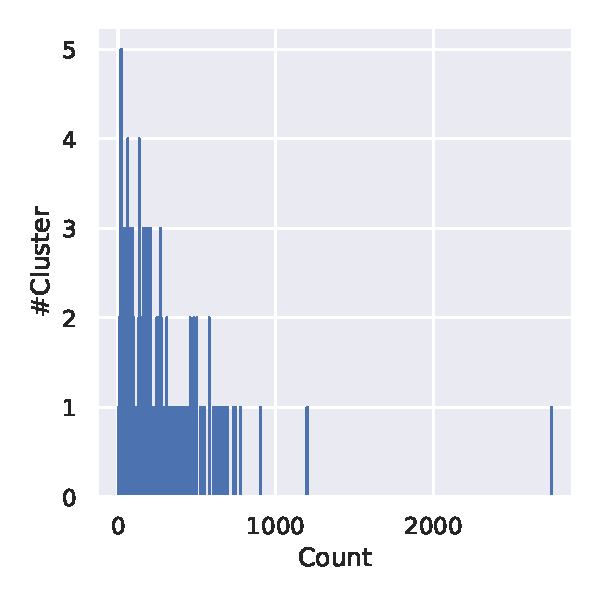
\includegraphics[width=\textwidth]{UMAP/Cluster_Distribution_Segment_4_alternative.pdf}
    \end{subfigure}
    \hfill
    \begin{subfigure}[b]{0.475\textwidth}
        \caption[Logarithmic Distribution]{\textbf{Logarithmic Distribution}}
        \label{subfig:UMAP_Cluster_DBCV_Distribution_log_4}            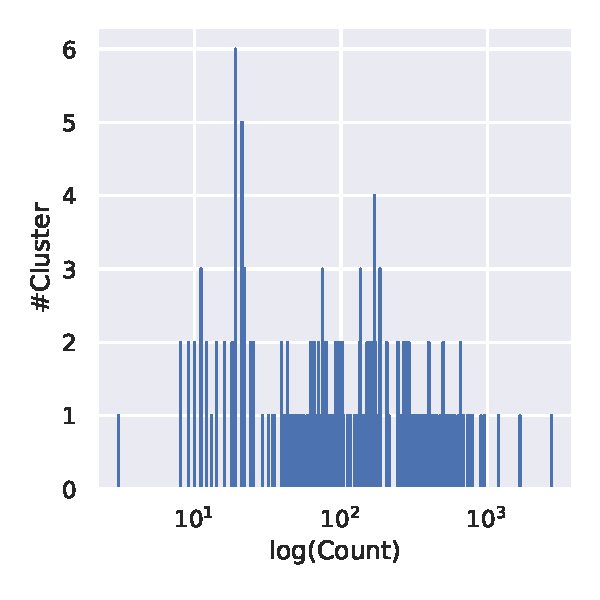
\includegraphics[width=\textwidth]{UMAP/Cluster_Distribution_Log_Segment_4_alternative.pdf}
    \end{subfigure}
    %\end{adjustbox}
    \caption[\Acrshort{DBCV} based Segment 4 Clustering (\Acrshort{UMAP})]{\textbf{\Acrshort{DBCV} based Segment 4 Clustering (\Acrshort{UMAP}).}.}
    \label{fig:UMAP_Cluster_DBCV_4}
\end{figure}

The cluster sized using \gls{UMAP} are spreaded more equally with no cluster of 3000 sequences or more. The only difference between the methods of \gls{PCA} and \gls{UMAP} ist the additional use of \gls{UMAP} after \gls{PCA} in the latter one (\autoref{sec:UMAP}). Therefore the difference in cluster size distribution must be caused by \gls{UMAP}. \gls{UMAP} not only reduces the dimension of the data but also changes the position of the points in the embedded dimension according to the used settings. The \colorbox{backcolour}{n\_neighbors=100} setting is most likely the cause of a change of this magnitude. By increasing the number of neighbors the points were more crowded in groups to support a bigger picture of the data in the embedded dimension and therefore build more clusters of equal sizes. Retrospective to the distribution of segment 4 sequences in the data in \autoref{fig:Frequency_4} it was expected, that a distribution of cluster sizes in segment 4 clustering would approximate the distribution of the sequences in the former one. Therefore a clustering with \gls{PCA} seems to give the expected results and appears as the best method for \gls{IAV} clustering. However this is only valid in combination with the use of the Kneedle Algorithm $\varepsilon$ exploration. The combination with the \gls{DBCV} is mostly irrelevant at this point, since as mentioned earlier, this results in only \gls{HDBSCAN} clustering without hybrid component for most segments and is therefore in any case not suitable for the proposed approach. 

% Also the distribution of cluster sizes seems to be more balanced e.~g.~ segment 4 (\autoref{subfig:UMAP_Cluster_Knee_Distributione_4} and \autoref{subfig:UMAP_Cluster_Knee_Distribution_log_4}) than in the \gls{PCA} approach (\autoref{subfig:PCA_Cluster_Knee_Distributione_4} and \autoref{subfig:PCA_Cluster_Knee_Distribution_log_4}) which could also contribute to the hybrid clustering by \gls{DBSCAN} alone. With a more distributed number of sequences in the clusters, less very small and very big clusters exist and overall more points are collected in small groups which decreases the chance for single points unaffected by the $\varepsilon$ threshold. 

Clustering by the method using \gls{PCA} in combination with the Kneedle Algorithm results also in the cluster-tree \autoref{fig:PCA_Cluster_Knee_4}. Coloring of the tree is based on the \gls{HA} antibody subtype as shown in \autoref{fig:Frequency_4}. If a cluster only contains sequences of one subtype, plus possibly some not classified sequences, the not classified sequences are declared as the subtype to. That way a clear presentation of the subtype distribution was possible, since the not classified sequences are very likely to actually belong to an existing subtype. If they don't belong to a existing subtype a cluster only containing these not classified sequences would most likely have occurred, which is not the case. Furthermore the chance to eventually break the classification of subtypes by declaring not classified sequences to a existing subtype is not given as the clusters are not based on subtypes in any way and the visualization is only for guidance and not possible for any segments other than 4 and 6 anyway. If a cluster contains sequences of more than one subtype plus possibly some not classified sequences, no coloring was performed, since the cluster is not homogeneous for one subtype and a declaration of the unclassified isn't possible to. The prime example for this is the yellow colored cluster 0 of subtype H9 (\autoref{fig:PCA_Clusteree_Knee_4} \textbf{\textsf{A}}). While all sequences are accumulated in this single cluster, the cluster size of 1569 is bigger than the number of H9 sequences in \autoref{fig:Frequency_4} with 1454. This is justified by the presence of 115 not classified sequences in the cluster which are declared as H9 since only H9 and unclassified sequences are present in the cluster.

The number of clusters for a given subtype of \gls{HA} antibody seems to correspond roughly to the overview of sequences in \autoref{fig:Frequency_4}. While very low represented subtypes like H15 is only represented by one cluster, containing all the 14 sequences, are high represented subtypes like H1 and H3 spreaded over more clusters.

\begin{figure}[!hbt]
    \centering
    \begin{tikzpicture}
        \node[anchor=south west,inner sep=0] (image) at (0,0) {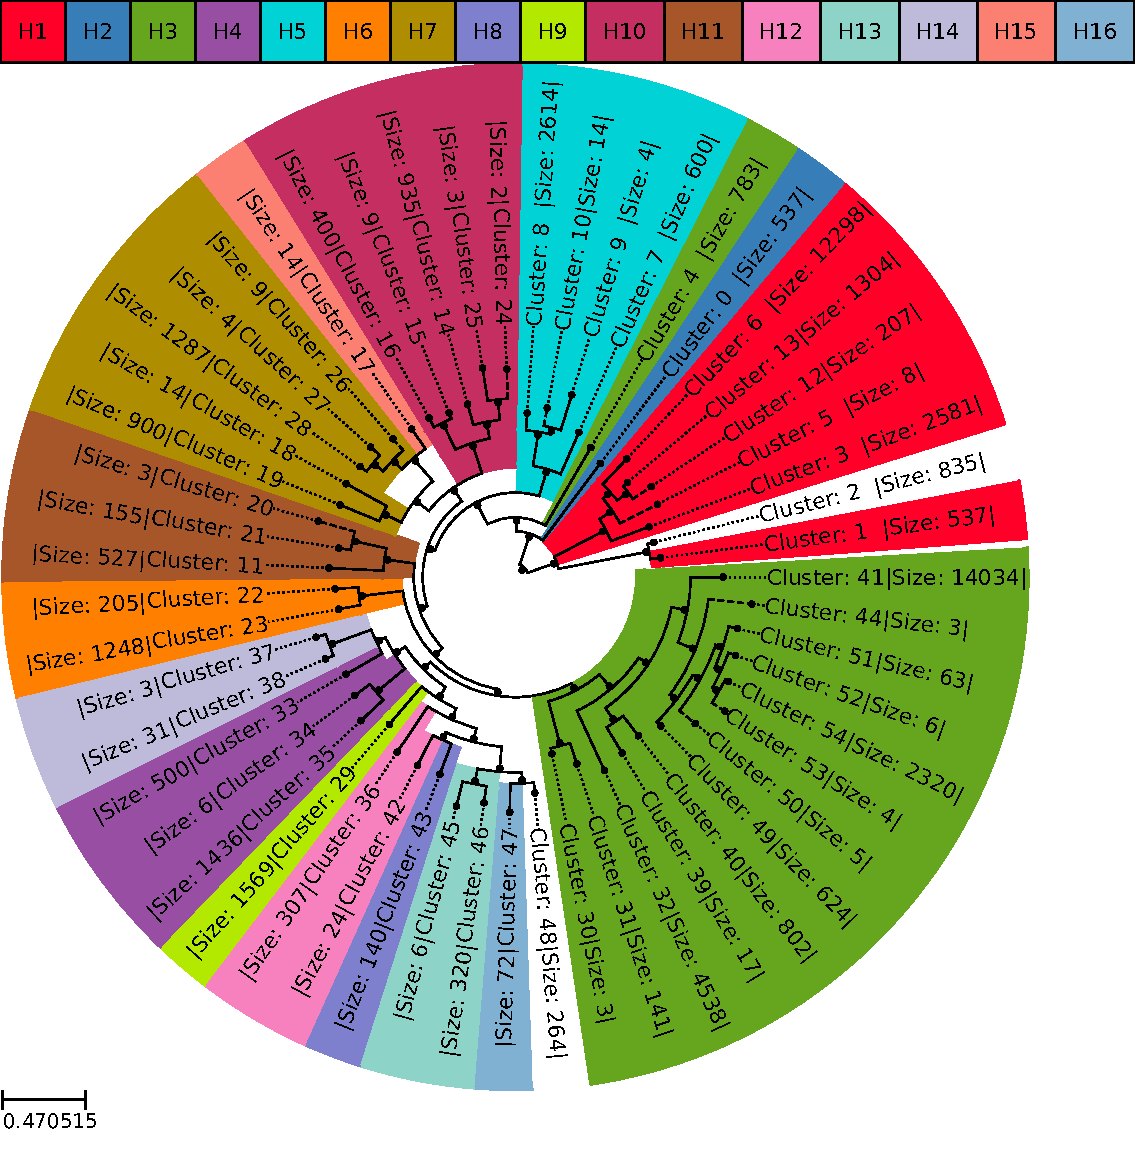
\includegraphics[width=\textwidth]{PCA/Clustertree_Segment_4_H_Knee.pdf}};
        \begin{scope}[x={(image.south east)},y={(image.north west)}]
            %\draw[help lines,xstep=.1,ystep=.1] (0,0) grid (1,1);
            \node at (0.15,0.16) [arrowstyle=1.5cm, anchor=east] {\textbf{\textsf{A}}};
            \node at (0.5,0.09) [arrowstyle=1.5cm, anchor=east, rotate=135] {\rotatebox{225}{\textbf{\textsf{B}}}};
            \node at (0.9,0.62) [arrowstyle=1.5cm, anchor=east, rotate=225] {\rotatebox{135}{\textbf{\textsf{C}}}};
            \node at (0.7,0.9) [arrowstyle=1.5cm, anchor=east, rotate=180] {\rotatebox{180}{\textbf{\textsf{D}}}};
        \end{scope}
    \end{tikzpicture}

    \caption[Knee based Segment 4 Clustertree (\Acrshort{PCA})]{\textbf{Knee based Segment 4 Clustertree (\Acrshort{PCA}).} .}
    \label{fig:PCA_Clusteree_Knee_4}
\end{figure}

Striking anomalies divergent from the expected nearly uniform allocation of the subtypes in \autoref{fig:PCA_Cluster_Knee_4} are noted by \textbf{\textsf{B}}, \textbf{\textsf{C}} and \textbf{\textsf{D}} and are discussed in the following. 
